\chapter{Linear Models}    
\label{chap:linmod}   

In Section \ref{rholargesmall} we made reference to \textit{linear
models}.  Directly or indirectly, they form the basis for much of ML.

\section{Minimizing MSPE}

Suppose we are predicting a random variable $Y$, based on a random
vector $X$, say predicting weight from (height,age).  Our guess will be
some function of $X$, $g(X)$.  What is the best $g$, in the sense of
minimizing MSPE?  In other words, how should we choose $g$ to minimize

\begin{equation}
\label{mspe}
E \left ( [Y - g(X)]^2 \right )
\end{equation}

% Using the Law of Iterated Expectations (Section \ref{adamsrule}), the
% above expression is equal to
% 
% \begin{equation}
% E \left [ E \left ( [Y - g(X)]^2 | X \right ) \right ]
% \end{equation}
% 
% For any random variable $W$, $E[ (W - c)^2$ is minimized by $c =
% EW$.\footnote{Write out the quantity as $E(W^2) -2c EW + (EW)^2$, then
% minimize with respect to $c$.}  Applying that to
% $E \left ( [Y - g(X)]^2 | X \right ) $, we have that:

One can show that:

\begin{quote}
We get minimum MSPE by taking $g(X)$ to be the conditional mean, $E(Y|X)$.
\end{quote}

This should make good intuitive sense:  To predict the weight of
someone 70 inches tall, we take our guess to be the mean weight of all
70-inch-tall people.

We will then define the \textit{regression function}

\begin{equation}
\mu(t) = E (Y | X = t)
\end{equation}

Note that the argument $t = (t_1,...,t_p)'$ is a vector.  (Note:  All
vectors will be column vectors if not otherwise stated.)
Also, prepending a 1, we will use the notation $\widetilde{t} = (1,t')'$.

This definition is \textit{general}; it does not assume a linear model.
Let's now see where the classical linear model comes from.

\section{Motivation for the Classical Linear Model}

Say we are predicting a variable $Y$ from $p$ features, $X_1,...,X_p$.
Let $X$ denote the (column) vector of those features.  Sometimes we will
also add a constant 1 at the beginning, setting

\begin{equation}
\widetilde{X} = (1,X_1,...,X_p)' 
\end{equation}

Here is the main point:

\begin{quote}
Suppose $(X,Y)$ has a $p+1$ dimensional normal distribution.  Then
the conditional distribution of $Y$ given $X$ has the following
properties:

\begin{itemize}

\item \textbf{Linearity:} 

\begin{equation}
\label{betadef}
\mu(t) = \beta_0 + \beta_1 t_1 + ... + \beta_p t_p  = \beta' \widetilde{t}
\end{equation}

for a certain vector ${\beta}$.\footnote{One can show that
$\beta = E(Y \widetilde{X}) [ E( \widetilde{X} \widetilde{X}') ]^{-1}$.}

\item \textbf{Conditional normality:}  For any $t$, the conditional
distribution of $Y$ given $X = t$ is normal.

\item \textbf{Homoskedasticity:}  The conditional
variance of $Y$ given $X = t$ is the same for all $t$.

\end{itemize} 

\end{quote}

\section{Coming Back Down to Earth}

For those readers who have some background in linear regression modeling, 
the above three bullet items will sound familiar.  They are the
motivation for the classic assumptions of linear modeling:  linearity,
normality and homoskedasticity.  \textit{However, note the following:}

\begin{itemize}

\item The normality and homoskedasticity assumptions are used only for
\textit{statistical inference}, i.e.\ confidence intervals and tests.
We will not be performing statistical inference in this
book; ML is mainly about \textit{prediction}.\footnote{Sadly, in ML
circles, the situation is confused by using the term \textit{inference}
for prediction.}  

Even for inference, those assumptions aren't really
necessary.  We get normality for our estimated $\beta$ from
the Central Limit Theorem, and we can deal with the lack of
homoskedasticity by using the \textit{sandwich estimator}, e.g.\ in the
R \textbf{sandwich} package. 

\item Many regresssion functions in practice are approximately linear.
And, as will be seen shortly, polynomial models, which may provide a
good fit in nonlinear situations, are actually linear!

\end{itemize} 

In other words:

\begin{quote}

\begin{itemize}

\item The classic linear model is motivated by settings in $(X,Y)$
has a multivariate normal distribution.

\item This assumption is highly restrictive, but \textit{is not
necessary} for our purposes.

\end{itemize} 

\end{quote}

For the remainder of this chapter, we assume 

\begin{equation}
\label{linassump}
g(t) = \beta' \widetilde{t}
\end{equation}

for some vector $\beta$ to be estimated from our data.

\section{Estimating $\beta$}

Here we lay groundwork leading up to the famous \textit{least-squares
estimate}.

\section{Sample vs.\ Population}

Most readers have probably noticed that when the results of a survey are
released, say during elections, a \textit{margin of error} (MOE) is stated.
For instance, ``55\% of those surveyed say they plan to vote for
Candidate Jones, with a margin of error of 3.2\%.''  The MOE is
recognition of the fact that only a sample of voters were surveyed, not
the entire population of voters.

Let $p$ denote the population proportion, i.e.\ the proportion of voters
across the population who favor Jones.  The value of $p$ is unknown, but
our estimate is $\widehat{p} = 0.55$.  The ``hat'' notation $\widehat{}$
means ``estimate of.''  (The MOE is the radius of a 95\% confidence
interval for $p$, though as noted, we do not make much use of statistical
inference in this book.)

Every ML method is an estimator in some form or other.  However, the
terms \textit{sample} and \textit{population} are not used in the ML
community.  Instead, they speak a \textit{probabilistic generative
process} to mean the same thing as sampling data from a population.

So, $\beta$ is a population value.  Its estimator from the data is
denoted $\widehat{\beta}$.

\subsection{The Least Squares Estimator}

Denote our data by $(X_{ij},Y_j), ~ j = 1,...,n$.  In other words, we
have $n$ data points, and in the $j^{th}$ of them, $X_{ij}$ and $Y_j$
are the valus of $X_i$ and $Y$, respectively.  Also, define

\begin{equation}
X^{(j)} = (1,X_{1j},...,X_{pj})'
\end{equation}

To keep a concrete example in mind, again suppose we are predicting
human weight $Y$ from height $X_1$ and age $X_2$.  $X^{(3)}$, for
instance, is then the vector (height,age) for the third person in our
data (with a 1 prepended).

Putting together the fact that $g$ minimizes (\ref{mspe}) and the
assumption (\ref{linassump}), we have that $\beta$ is the vector $b$ 
that minimizes

\begin{equation}
\label{linmspe}
E \left [ (Y - b' \widetilde{X})^2 \right ]
\end{equation}

The sample analog of this quantity is

\begin{equation}
\label{sammspe}
\frac{1}{n}
\sum_{j=1}^n \left [ (Y_j - b' X^{(j)})^2 \right ]
\end{equation}

Since $b = \beta$ minimizes (\ref{linmspe}), it is natural by analogy to
take $\widehat{\beta}$ to be the value of $b$ that minimizes
(\ref{sammspe}).

Just a little bit more notation:

\begin{equation}
D = (Y_1,...,Y_n)'
\end{equation}

\begin{equation}
A = 
\left (
\begin{array}{r}
X^{(1)'} \\
... \\
X^{(n)'} \\
\end{array}
\right )
\end{equation}

Then (\ref{sammspe}) (without the $1/n$ factor) is

\begin{equation}
\label{quad}
(D - Ab)'(D - Ab)
\end{equation}

To minimize this, we must set the derivative of (\ref{quad}) to 0.  It
can easily be verified that for a vector $u$, 

\begin{equation}
\frac{d}{du} u'u = 2u
\end{equation}

Applying this and the Chain Rule to (\ref{quad}), i.e.

\begin{equation}
\frac{d}{db} = \frac{d}{du} ~ \frac{du}{db}
\end{equation}


we have

\begin{equation}
0 = A' (D - Ab) 
\end{equation}

Solve for $b$:

\begin{equation}
\label{ols}
\widehat{\beta} = (A'A)^{-1} A'D
\end{equation}

This is the \textit{least squares estimator} of $\beta$.

\section{Computation}

We certainly do not want to do this compution by hand.  What are our
choices?

\subsection{lm()}

R's \textbf{lm()} (``linear model'') function does the computation for
us.  Here is an example using \textbf{mlb}, a dataset in the
\textbf{regtools} package, involving Major League Baseball
players:\footnote{We trimmed down the number of columns here.}

\begin{lstlisting}
> head(mlb)  # take a look around
        Position Height Weight   Age
1        Catcher     74    180 22.99
2        Catcher     74    215 34.69
3        Catcher     72    210 30.78
4  First_Baseman     72    210 35.43
5  First_Baseman     73    188 35.71
6 Second_Baseman     69    176 29.39
> lmout <- lm(Weight ~ Height + Age,mlb)
> coef(lmout)
 (Intercept)       Height          Age 
-187.6381754    4.9235994    0.9115326 
> predict(lmout,data.frame(Height=73,Age=25))
       1 
194.
\end{lstlisting}

The call says, ``Fit a linear model for predicting weight from height
and age, using the dataset \textbf{mlb}.''  The \textbf{coef()} function
extracts $\widehat{\beta}$ from the output object.  We see that
$\widehat{\beta} = (-187.64,4.92,0.91)'$. 

We then predict a new case.  If the player whose weight is to be
predicted is of height 73 and age 25, we would predict wieght 194 (an
integer here just by coincidence).

By the way, \textbf{coef()} and \textbf{predict()} are \textit{generic}
functions in R, meaning that their actions depend on the class of object
they are called on.  In this case, \textbf{lmout} is of class
\textbf{'lm'}, so \textbf{coef()} is \textit{dispatched} to a function
\textbf{coef.lm()} tailored to such objects; \textbf{predict()} is
dispatched to \textbf{predict.lm()}.  There are many generic functions
in R, notably \textbf{print()} and \textbf{plot()}.

\subsection{qeLin()}

In this book, we will use the \textbf{qeML} package.  The name stands
for ``quick and easy machine learning,'' alluding to the goal of making
things as quick and convennient as possible:

\begin{itemize}

\item The functions have a simple, \textit{uniform} user interface.

\item Cross-validation is automatically taken care of .

\end{itemize} 

Most of the \textbf{qeML} functions are wrappers to functions in other R
packages; \textbf{qeML} adds a simple, uniform interface to them.

Let's apply it to the above example:

\begin{lstlisting}
> qeout <- qeLin(mlb[,-1],'Weight')
holdout set has  101 rows
\end{lstlisting}

The \textbf{qeML} functions all have the user specify the ``Y'' variable
in the second argument, and ``X'' in the first argument.  It is assumed
that all of the ``X'' columns will be used to predict ``Y,'' so to be
consistent with the earlier example, we needed to exclude column 1.

We can predict with any of the \textbf{qeML} functions.

\begin{lstlisting}
> predict(qeout,data.frame(Height=73,Age=25))
      11 
194.2245 
\end{lstlisting}

The functions do automatic cross-validation, with the size of the
holdout being 10\% of the size of the dataset.\footnote{This is the
reason for the slight discrepancy above.} The prediction accuracy on the
holdout set is in the \textbf{testAcc} component of the return value:

\begin{lstlisting}
> qeout$testAcc
[1] 14.13652
\end{lstlisting}

For continuous ``Y,'' this is the Mean Absolute Prediction Error
(MAPE).  On average, our predictions are about 14 pounds off.
Could this be improved by adding \textbf{Position} to our feature set?

\begin{lstlisting}
> qeLin(mlb,'Weight')$testAcc
holdout set has  101 rows
[1] 12.16986
\end{lstlisting}

Ah, yes.  Catchers tend to be stocky, pitchers lanky and so on, so there
is valuable extra information there.  

\subsection{Dumy/One-Hot Variables}

By the way, \textbf{lm()} automatically converts R factors to
\textit{dummy/one-hot} form,\footnote{The term \textit{dummy variables }
is used in statistics, economics and almost all fields of application,
but in the machine learning world, the term is \textit{one-ot}.} as was
the case for \textbf{Position} here.  This is necessary for the matrix
operations on which the linear model is based, which of course are
numeric. 

So, if we have a categorical variable with $k$ categories ($k =8$
here\footnote{There are 9 positions in baseball, but the dataset has a
slightly different classification, e.g.\ just one Outfielder
category.}), we create $k-1$ dummies.  We lose no information that
way---if a record is not in those $k-1$ categories, it must be in the
$k^{th}$---and it is actually necessary.  Here is why:

If we had dummy columns for all $k$ categories, the sum of those columns
would be a vector of all 1s.  But our matrix $A$ has a column of 1s
already.  Thus the columns would be linearly dependent.  But then $A$
would not be full rank, and $A'A$ would have the same problem.  The
later matrix would then be nonintertible, making (\ref{ols}) impossible.

\subsection{Uniform APIs in qeML}

As noted, the \textbf{qeML} functions offer the benefit of a uniform
API.  Let's try the kNN (``k-nearest neighbors'' method:

\begin{lstlisting}
> qeKNN(mlb,'Weight')$testAcc
holdout set has  101 rows
[1] 15.05624
\end{lstlisting}

Oh, not as good.  If the true regression function is approximately
linear, we generally will do better by exploiting that fact.

As wrappers, the class of a \textbf{qeML} return value is a subclass of
the function being wrapped:

\begin{lstlisting}
> class(qeout)
[1] "qeLin" "lm"   
\end{lstlisting}

They thus inherit methods:

\begin{lstlisting}
> coef(qeout)
 (Intercept)       Height          Age 
-192.0942868    4.9726027    0.9327504 
\end{lstlisting}

\section{The Logistic Model}

Say we are predicting a binary``Y.''  In the \textbf{mlb} data, say we
are predicting whether a player is a catcher.  Say we define $Y$ to be 1
for catcher, 0 if not.  In many ML circles, the coding is 1 and - 1, as
opposed to the ``statistical'' 1,0.  The latter has the advantage that
its expectation is the probability of the $Y = 1$ class, which will be
seen below is an integral part of the \textit{logistic} model

\begin{equation}
\mu(t) = E(Y | X= t) = P(Y = 1 | X = t)
\end{equation}

The model is

\begin{equation}
\label{logit}
P(Y = 1 | X = t) =
\frac{1}{1 + e^{-\beta' t}}
\end{equation}

The reader will notice that in that expression we see the expression
$\beta't$ from the linear model.  Accordingly, the logistic (often
called ``logit'') is termed a \textit{generalized linear model}.
The R \textbf{glm()} function implements models such as this.  (Another
is \textit{Poisson regression}.)  In the logistic case,
\textbf{qeLogit()} serves as a wrapper.

\subsection{Again, a Multivariate Normal Motivation}

The right-hand side of (\ref{logit}) is in (0,1), and thus a reasonable
model for a probability.  It is an increasing function of $\beta't$,
thus giving it an appealing quasi-linear nature.  If say $Y$ codes
having diabetes, it is reasonable to postulate that the probability of
having the disease is an increasing function of the age of the patient.

As with the linear model, though, there is a multivariate normal
motivation:

\begin{quote}
Suppose the distribution of $X$, given $Y = i$, is multivariate normal
with mean vector different for each $i$ but with covariance matrix being
the same across values of $i, i = 0,1$.  Then (\ref{logit}) holds.
\end{quote}

Let's see how this works for $p = 1$.  Consider a short interval in the
real line, $A = (t,t+\epsilon)$.  We'll look at $P(Y = 1 | X \textrm{ in
} A)$, then let $\epsilon \rightarrow 0$ to get $P(Y = 1 | X = t)$

Let $q = P(Y = 1)$, the \textit{unconditional} probability of class 1.
Let $w_i(t)$ denote the conditional density of $X$, given $Y = i$ (which
by assumption is normal).  Then by Bayes Rule,

\begin{eqnarray}
P(Y = 1 | X \textrm{ in } A) [&=& 
\frac
{q P(X \textrm{ in } A ~|~  Y = 1)}
{
{q P(X \textrm{ in } A ~|~ Y = 1)} +
(1-q) P(X \textrm{ in } A ~|~ Y = 0) 
} \\
&\approx&  
\frac{q \epsilon w_1(t)}
{q \epsilon w_1(t) + (1-q) \epsilon w_0(t)} \\
&=& 
\label{logitform}
\frac{1}{1 + \frac{1-q}{a} \frac{w_0(t)}{w_1(t)}}
\end{eqnarray}

Now, since the $w_i$ are normal, we have

\begin{equation}
w_i(t) = 
\frac{1}{\sqrt{2 \pi} \sigma}
% e^{- \left ( z \right )^2}
e^{-0.5 \left ( \frac{t-\mu_i}{\sigma} \right )^2}
\end{equation}

Substituting this in (\ref{logitform}) does indeed simplify to
(\ref{logit}) for the appropriate $\beta$.

\subsection{Example:  Predicting ``Catcherness''}

\begin{lstlisting}
> catch <- mlb$Position == 'Catcher'
> mlb$catch <- as.factor(catch)
> qeo <- qeLogit(mlb[,-1],'catch')
> predict(qeo,data.frame(Height=73,Weight=225,Age=25))
$predClasses
[1] "FALSE"

$probs
         FALSE      TRUE
[1,] 0.8743196 0.1256804
\end{lstlisting}

The \textbf{qeML} functions sense that $Y$ is binary (or more generally,
categorical) by testing whether it is an R factor.  So we needed to
convert the logical vector to a factor.  The prediction was FALSE, i.e.\
this player is guessed to not be a catcher, and in fact has only about a
13\% chance of being a catcher.

\subsection{Example:  Vertebral Disease}

As noted, we can also predict general categorical $Y$.  Here we
consider a vertebral dataset from the UCI Machine Learning Repository.

\begin{lstlisting}
> head(vert)
     V1    V2    V3    V4     V5    V6 V7
1 63.03 22.55 39.61 40.48  98.67 -0.25 DH
2 39.06 10.06 25.02 29.00 114.41  4.56 DH
3 68.83 22.22 50.09 46.61 105.99 -3.53 DH
4 69.30 24.65 44.31 44.64 101.87 11.21 DH
5 49.71  9.65 28.32 40.06 108.17  7.92 DH
6 40.25 13.92 25.12 26.33 130.33  2.23 DH
\end{lstlisting}

There are three disease types, NO, DH and SL, where NO means normal.
The other columns are various vertebral meansurements.

Our previous example and discussion concerned binary $Y$.  Here $Y$
as three categories.  How does \textbf{qeLogit()} handle this?  It takes
the \textit{One vs.\ All} approach::

\begin{itemize}

\item Create three separate dummy/one-hot variables from $Y$, one each
for NO, DH and SL. 

\item Fit a logit model for predicting NO from V1,...,V6.

\item Fit a logit model for predicting DH from V1,...,V6.

\item Fit a logit model for predicting SL from V1,...,V6.

\item Then, for any future case, form predictions for it from all three
models.  Whichever model gives the highest probability, take our
prediciton to be that category.

\end{itemize} 

\begin{lstlisting}
> qel <- qeLogit(vert,'V7')
holdout set has  31 rows
\end{lstlisting}

As an example of prediction, consider a patient like the one in
\textbf{vert[1,]}; but with $V7 = 1.88$.

\begin{lstlisting}
> newPatient <- vert[1,-7]
> newPatient$V6 <- 1.88
> predict(qel,newPatient)
$predClasses
[1] "DH"

$probs
            DH        NO         SL
[1,] 0.8594815 0.1190561 0.02146242
\end{lstlisting}

The prediction would be DH, with a probability of about 86\%.

How well does logit predict on this dataset?

\begin{lstlisting}
> qel$testAcc
[1] 0.1612903
> qel$baseAcc
[1] 0.5053763
\end{lstlisting}


For binary/categorical $Y$, the \textbf{qeML} functions report the
overall misclassification rate.  Here, we would predict correctly about
84\% of the time. 

Are the features very helpful in prediction?  Consider this:

\begin{lstlisting}
> table(vert$V7) / nrow(vert)

       DH        NO        SL 
0.1935484 0.3225806 0.4838710 
\end{lstlisting}

If we did not have the features to use for prediction, we would always
guess SL, as it is the most common cateogory.  We would be right 48\% of
the time, thus wrong 52\% of the time.  But actually we didn't need to
make that calculation above; it's returned by \textbf{qeLogit()}:

\begin{lstlisting}
> qel$baseAcc
[1] 0.5053763
\end{lstlisting}

(Again, The small discrepancy is due to using the full dataset versus
using just the training set.)

\section{Polynomial Models}

Recall Figure \ref{mightlintrend}, reproduced below for convenience:

% \begin{figure}
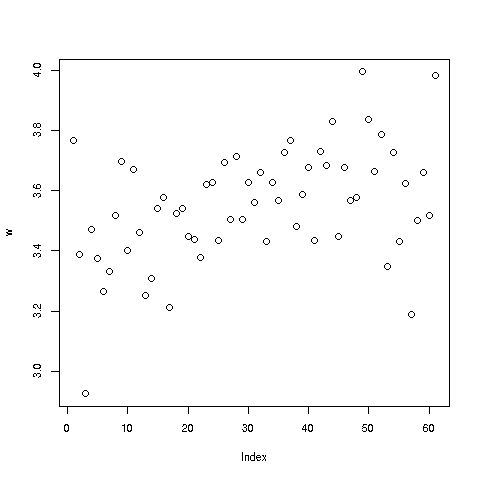
\includegraphics[width=3.5in]{Images/MeanRatVsAge.png}
% \caption{Rating vs.\ Age}
% \end{figure}

The trend seemed to be vaguely linear, upward, but maybe even a downward
trend near the end.  The latter point suggests there may even be a
quadratic trend, with the middle-aged given higher ratings while the
young and old are less generous.

Though it sounds counterintuitive, quadratic models are actually linear!
Here is why:  The model is

\begin{equation}
\label{firstquad}
E( \textrm{userMean} ~|~ \textrm{age} = t) =
\beta_0 + \beta_1 \textrm{ age} + \beta_2 \textrm{ age}^2
\end{equation}

This is quadratic in age but linear in $\beta$.  For instance, if we
were to multiply each $\beta_i$ by 2.4, the entire sum would grow by
that factor.

Indeed, we should just consider $\textrm{age}^2$ as a new feature:

\begin{lstlisting}
> z <- ml100kpluscovs[,c('age','userMean')] 
> z$age2 <- z$age^2
> head(z)
  age userMean age2
1  24 3.610294  576
2  20 3.918605  400
3  27 3.393720  729
4  25 3.470046  625
5  33 4.025271 1089
6  28 3.993007  784
\end{lstlisting}

We would then run \textbf{qeLin()} as usual:

\begin{lstlisting}
> qeLin(z,'userMean')$testAcc
holdout set has  1000 rows
[1] 0.3254251
> qeLin(z[,1:2],'userMean')$testAcc
holdout set has  1000 rows
[1] 0.3472223
\end{lstlisting}

There may be a slight improvement of the quadratic model over the linear
one.  But we must remember that since the holdout set is randomly
chosen, there is some randomness to the above numbers.  Let's try 10
replications of each, using the \textbf{replicMeans()} function from the
\textbf{regtools} package:

\begin{lstlisting}
> replicMeans(10,"qeLin(z[,1:2],'userMean')$testAcc")
holdout set has  1000 rows
holdout set has  1000 rows
holdout set has  1000 rows
holdout set has  1000 rows
holdout set has  1000 rows
holdout set has  1000 rows
holdout set has  1000 rows
holdout set has  1000 rows
holdout set has  1000 rows
holdout set has  1000 rows
[1] 0.3363623
attr(,"stderr")
[1] 0.003186719
> replicMeans(10,"qeLin(z,'userMean')$testAcc")
holdout set has  1000 rows
holdout set has  1000 rows
holdout set has  1000 rows
holdout set has  1000 rows
holdout set has  1000 rows
holdout set has  1000 rows
holdout set has  1000 rows
holdout set has  1000 rows
holdout set has  1000 rows
holdout set has  1000 rows
[1] 0.3392382
attr(,"stderr")
[1] 0.003183424
\end{lstlisting}

(The \textit{standard error} is the estimated standard deviation of the
reported mean.)

The quad model probably is not helpful here.

A better example is the \textbf{pef} dataset from \textbf{regtools}.

\begin{lstlisting}
> head(pef)
       age     educ occ sex wageinc wkswrkd
1 50.30082 zzzOther 102   2   75000      52
2 41.10139 zzzOther 101   1   12300      20
3 24.67374 zzzOther 102   2   15400      52
4 50.19951 zzzOther 100   1       0      52
5 51.18112 zzzOther 100   2     160       1
6 57.70413 zzzOther 100   1       0       0
\end{lstlisting}

This is data from the 2000 US census, in Silicon Valley, over six
different computer-related occupations.  Let's try a linear model:

\begin{lstlisting}
> qeLin(pef,'wageinc')$testAcc
holdout set has  1000 rows
[1] 25906.99
\end{lstlisting}

On average, our prediction is off by almost \$26,000.  But it's better
than not using the features at all, i.e.\ just using mean income as our
predictor:

\begin{lstlisting}
> qeLin(pef,'wageinc')$baseAcc
holdout set has  1000 rows
[1] 30804.21
\end{lstlisting}

Let's try a quadratic model.  But it would be harder than
(\ref{firstquad}).  We would have to add columns for squares of all the 
variables (first converting the categorical variables like \textbf{occ} 
do dummies/one-hots), \textit{and} computer ``cross-product terms, such
as age times sex (representing a difference in effect of age, between
men and wome).

But \textbf{qeML} does all that for us, via \textbf{qePolyLin()}.  So,
let's try that:

\begin{lstlisting}
> replicMeans(50,"qeLin(pef,'wageinc')$testAcc")
[1] 25361
attr(,"stderr")
[1] 145.1841
> replicMeans(50,"qePolyLin(pef,'wageinc',deg=2)$testAcc")
[1] 24762.21
attr(,"stderr")
[1] 136.9662
\end{lstlisting}

So, a quadratic model yields a small, but likely worthy, improvement.

There is also \textbf{qePolyLog()}, for quadratic features in a logistic
model.

\section{Application to Collaborative Filtering}

So, let's make our first attempt at collaborative filtering, on the
MovieLens data.  We'll just use a linear model, with the small 100K
dataset.

\begin{lstlisting}
> qeLin(ml100kpluscovs[,c('user','item','rating')],'rating')$testAcc
holdout set has  1000 rows
[1] 0.9213201
> qeLin(ml100kpluscovs[,c('user','item','rating')],'rating')$baseAcc
holdout set has  1000 rows
[1] 0.9523251
> qeLin(ml100kpluscovs[,c('rating','userMean','itemMean')],'rating')$testAcc
holdout set has  1000 rows
[1] 0.7484943
\end{lstlisting}

Remember, \textbf{lm()}, and thus the wrapper \textbf{qeLin()}, will
convert the \textbf{user} variable to dummies, and the same for
\textbf{item}.  With 943 users and 1682 items, that's 2624 dummies.
A rough rule of thumb is that one should have at most $p < \sqrt{n}$, i.e.\
about 300 features.  In other words, using the \textbf{user} and
\textbf{item} columns is probably overfitting.  Replacing them by the
\textit{embeddings}, i.e.\ replacing a variable by its summary or proxy,
seems to be a good idea here; replacing 2624 columns by 2 seemed to pay
off.

\section{Regularization: the LASSO}

A number of modern statistical methods ``shrink'' their classical
counterparts.  This is true for ML methods as well.  In particular, the
principle may be applied in:

\begin{itemize}

\item Boosting.

\item Linear models.

\item Support vector machines.

\item Neural networks.

\end{itemize}

This is also applied to some RS models, such as matrix factorization.

\subsection{Motivation}

Suppose we have sample data on human height, weight and age.  Denote the
population means of these quantities by $\mu_{ht}$, $\mu_{wt}$ and
$\mu_{age}$.  We estimate them from our sample data as the corresponding
sample means, $\overline{X}_{ht}$, $\overline{X}_{wt}$ and
$\overline{X}_{age}$.

Just a bit more notation, giving names to vectors:

\begin{equation}
\mu = (\mu_{ht},\mu_{wt}, \mu_{age})
\end{equation}

\noindent
and

\begin{equation}
\overline{X} = (\overline{X}_{ht},\overline{X}_{wt}, \overline{X}_{age})
\end{equation}

\noindent
Amazingly, \textit{James-Stein theory} says
the best estimate of $\mu$ might NOT be $\overline{X}$.\footnote{Here
``best'' means in terms of Mean Square Error.  The MSE for the
non-shrunken case is $E \left [||\overline{X} - \mu ||^2 \right ].$}  
It might be a shrunken-down version of $\overline{X}$, say $0.9
\overline{X}$, i.e.

\begin{equation}
(0.9 \overline{X}_{ht},0.9 \overline{X}_{wt}, 0.9 \overline{X}_{age})
\end{equation}

\noindent
And the higher the dimension (3 here), the more shrinking needs to be done.
(Though for 1 or 2 dimensions, shrinkage brings no improvement.)
The intuition is this:  For many samples, there are a few data points
that are extreme, on the fringes of the distribution.  These points skew
our estimators, in the direction of being too large.  So, it is optimal
to shrink them.

How much shrinking should be done?  In practice this is unclear, and
typically decided by our usual approach, cross-validation.

Putting aside the mathematical theory --- it's quite deep --- the
implication for us in this book is that, for instance, the least-squares
estimator $\widehat{\beta}$ of the population coefficient vector $\beta$
in the linear model is often too large, and should be shrunken.  Most
interestingly, \textbf{this turns out to be a possible remedy for
overfitting}.

\subsection{Shrinking $\widehat{\beta}$ in Linear Regression Models}

Instead of finding the value of $b$ that minimizes (\ref{quad}), we
minimize

\begin{equation}
\label{quadLASSO}
(D - Ab)'(D - Ab) + \lambda ||b]]_{1}
\end{equation}

The value of the hyperparameter $\lambda > 0$ is up to the analyst, but
is typically chosen by cross-validation.  The resulting $\widehat{\beta}$
is called the Least Absolute Shrinkage and Selection Operator, LASSO.

Why does this result in shrinkage?  In minimizing (\ref{quad}) we are
given free rein, choosing any $b$ that we want.  But (\ref{quadLASSO})
penalizes us for using longer $b$.  Actually, one can show that
minimizing (\ref{quadLASSO}) is equivalent to minimizing (\ref{quad})
under the constraint that 

\begin{equation}
\label{dual}
||b||_{1} \leq \eta
\end{equation}

$\eta$ is now the hyperparameter.

\subsection{The Famous LASSO Picture}

As mentioned, a key property of the LASSO is that it usually provides a
\textit{sparse} solution for $\widehat{\beta}$, meaning the many of the
$\widehat{\beta}_i$ are 0.  In other words, many features are discarded,
thus providing a means of dimension reduction, thus an approach to
avoiding overfitting.  Figure \ref{lassosub} shows why.  Here is how it
works.

\begin{figure}
\vskip 0.2in
\centerline{
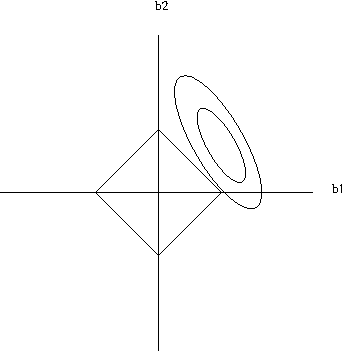
\includegraphics[width=2.75in]{Images/LASSO_gray.png}
}
\caption{Feature subsetting nature of the LASSO}
\label{lassosub}
\end{figure}

The figure is for the case of $p = 2$ predictors, whose coefficients are
$b_1$ and $b_2$.  (For simplicity, we assume there is no constant term
$b_0$.)  Let $U$ and $V$ denote the corresponding features.
Write $b = (b_1,b_2)$ for the vector of the $b_i$.

Without shrinkage, we would choose $b$ to minimize the sum of squared
errors,

\begin{equation}
\label{sse}
SSE = (Y_1 - b_1 U_1 - b_2 V_1)^2 + ... +
(Y_n - b_1 U_n - b_2 V_n)^2
\end{equation}

Recalling that the non-shrunken $b$ is called the Ordinary Least Squares
estimator, let's name that $b_{OLS}$, and name the corresponding SSE value
$SSE_{OLS}$.

The horizontal and vertical axes are for $b_1$ and $b_2$, as shown.  There is one ellipse for each possible value of SSE.  For SSE equal to, say 16.8, the corresponding ellipse is the set of all points $b$ that have SSE = 16.8. As we vary the SSE value, we get various concentric ellipses, two of which are shown in the picture.  The smaller the ellipse, the smaller the value of SSE.

The OLS estimate is unique, so the ellipse for SSE = $SSE_{OLS}$ is
degenerate, consisting of the single point $b_{OLS}$.

The corners of the diamond are at $(\eta,0)$, $(0,\eta)$ and so on.  Due
to the constraint (\ref{dual}), our LASSO estimator $b_{LASSO}$
must be somewhere within the diamond.

Remember, we want SSE --- the sum of square prediction errors --- to be
as small as possible, but at the same time we must stay within the
diamond.  So the solution is to choose our ellipse to just barely touch
the diamond, as we see with the outer ellipse in the picture.  The
touchpoint is then our LASSO solution, $b_{LASSO}$.

But that touchpoint is sparse --- $b2 = 0$!  And you can see that, for
almost any orientation and position of the ellipses, the eventual
touchpoint will be one of the corners of the diamond, thus a sparse
solution.  Thus the LASSO will usually be sparse, which is the major
reason for its popularity.

If we were to use the L2 norm in (\ref{quadLASSO}), that diamond would
be a circle.  The resulting $\widehat{\beta}$ is called the
\textit{ridge estimator}.  It also shrinks, but is not sparse, since the
touchpoint can be anywhere.

\subsection{The qeLASSO Function}

This wraps the \textbf{glmnet} package, which chooses $\lambda$ through
its own internal cross-validation.

